%----------------------------------------------------------------------------------------
%	PACKAGES AND OTHER DOCUMENT CONFIGURATIONS
%----------------------------------------------------------------------------------------

\documentclass[landscape,archE1,fontscale=0.285]{baposter} % Adjust the font scale/size here

\usepackage{graphicx} % Required for including images
\graphicspath{{figures/}} % Directory in which figures are stored

\usepackage{amsmath} % For typesetting math
\usepackage{amssymb} % Adds new symbols to be used in math mode

\usepackage{float}
\usepackage{booktabs} % Top and bottom rules for tables
\usepackage{enumitem} % Used to reduce itemize/enumerate spacing
\usepackage{palatino} % Use the Palatino font
\usepackage[font=small,labelfont=bf]{caption} % Required for specifying captions to tables and figures

\usepackage{multicol} % Required for multiple columns
\setlength{\columnsep}{1.5em} % Slightly increase the space between columns
\setlength{\columnseprule}{0mm} % No horizontal rule between columns

\usepackage{tikz} % Required for flow chart
\usetikzlibrary{shapes,arrows} % Tikz libraries required for the flow chart in the template

\newcommand{\compresslist}{ % Define a command to reduce spacing within itemize/enumerate environments, this is used right after \begin{itemize} or \begin{enumerate}
\setlength{\itemsep}{1pt}
\setlength{\parskip}{0pt}
\setlength{\parsep}{0pt}
}

\definecolor{lightblue}{rgb}{0.145,0.6666,1} % Defines the color used for content box headers

\begin{document}

\begin{poster}
{
headerborder=closed, % Adds a border around the header of content boxes
colspacing=1em, % Column spacing
bgColorOne=white, % Background color for the gradient on the left side of the poster
bgColorTwo=white, % Background color for the gradient on the right side of the poster
borderColor=lightblue, % Border color
headerColorOne=black, % Background color for the header in the content boxes (left side)
headerColorTwo=lightblue, % Background color for the header in the content boxes (right side)
headerFontColor=white, % Text color for the header text in the content boxes
boxColorOne=white, % Background color of the content boxes
textborder=roundedleft, % Format of the border around content boxes, can be: none, bars, coils, triangles, rectangle, rounded, roundedsmall, roundedright or faded
eyecatcher=true, % Set to false for ignoring the left logo in the title and move the title left
headerheight=0.175\textheight, % Height of the header
headershape=roundedright, % Specify the rounded corner in the content box headers, can be: rectangle, small-rounded, roundedright, roundedleft or rounded
headerfont=\Large\bf\textsc, % Large, bold and sans serif font in the headers of content boxes
%textfont={\setlength{\parindent}{1.5em}}, % Uncomment for paragraph indentation
linewidth=2pt % Width of the border lines around content boxes
}
%----------------------------------------------------------------------------------------
%	TITLE SECTION 
%----------------------------------------------------------------------------------------
%
{
\includegraphics[height=12em]{figures/Inst-Prim-FulClr.png}} % First university/lab logo on the left
{\bf\textsc{Computational Evalutions of Proton Induced Gain in a Portable Faraday Cup}\vspace{0.2em}} % Poster title
{\textsc{Shaun Marshall$^{1\dag}$, Blake Currier$^1$, Andrew Hodgdon$^2$ \\$^1$Department of Physics, Worcester Polytechnic Institute, Worcester, MA 01609\\ $^2$RadSim, LLC, Newton, MA 02462}} \\ % Author names and institution
%{
\includegraphics[height=4em]{logo.png}} % Second university/lab logo on the right

%----------------------------------------------------------------------------------------
%	INTRODUCTION
%----------------------------------------------------------------------------------------

\headerbox{Introduction}{name=introduction,column=0,row=0,above=bottom}{

\begin{itemize}[leftmargin=*]\compresslist
\item {\fontsize{15}{18}\selectfont Protons offer increasingly popular radiation therapy alternative via localized dose distribution}
\end{itemize}
\begin{center}
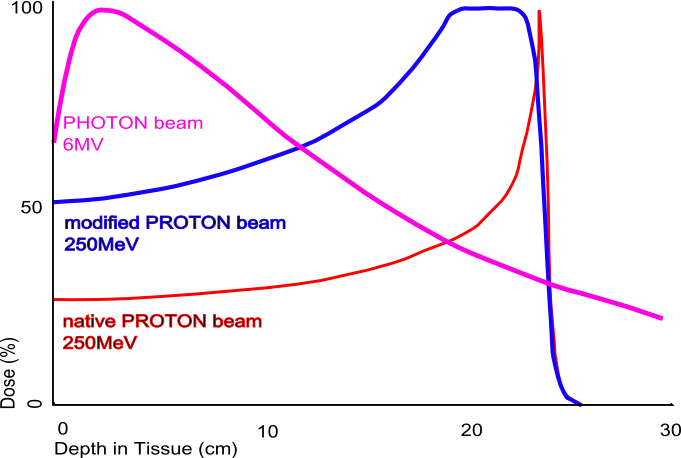
\includegraphics[width=0.75\linewidth]{figures/BraggPeak.png}
\captionof{figure}{Bragg Peak behavior of proton beam dosimetry.  Wikimedia File:BraggPeak.png.}
\end{center}
\begin{itemize}[leftmargin=*]\compresslist
\item {\fontsize{15}{18}\selectfont Calibration methods lack precision, esp. for pencil-beam scanning}
\item {\fontsize{15}{18}\selectfont Seek feasible (vacuumless, chamberless) solution for mid-range energies}
\item {\fontsize{15}{18}\selectfont Modeled after PMFC\cite{Gottschalk:1993,Gottschalk:2009}}
\end{itemize}
\begin{center}
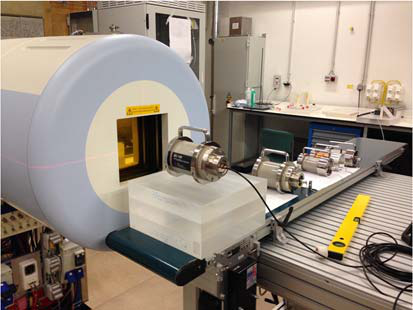
\includegraphics[width=0.75\linewidth]{figures/HIT_setup.png}
\captionof{figure}{Experimental beamline at Heidelberg Institute of Technology}
\end{center}
}

%----------------------------------------------------------------------------------------
%	MONTE CARLO SIMULATION
%----------------------------------------------------------------------------------------

\headerbox{Monte Carlo Simulation}{name=montecarlosimulation,column=1,row=0,aligned=introduction,above=bottom}{

{\fontsize{15}{18}\selectfont \textbf{Geant4 10.1-patch01}}
\begin{itemize}[leftmargin=*]\compresslist
\item {\fontsize{15}{18}\selectfont For each particle \emph{Track} i per Event j of N, tally net gain}
  $$ g_{ij} = \left\{\begin{array}{ll}
                  +q_i(Ne)^{-1}, & \text{if } q_i \rightarrow Cu \\
                  -q_i(Ne)^{-1}, & \text{if } q_i \leftarrow Cu \\
                  +q_id_\%(Ne)^{-1}, & \text{if } q_i \rightarrow KA(d_\%) \\
                  -q_id_\%(Ne)^{-1}, & \text{if } q_i \leftarrow KA(d_\%) \\
                  \end{array}\right.
  $$
\item {\fontsize{15}{18}\selectfont Charge defect} $\ = \sum_j^N \sum_i g_{ij} - 1$
\end{itemize}

{\fontsize{15}{18}\selectfont \textbf{Geometry Construction}}

\begin{table}[H]
  \centering
  \caption{Cylindrical definitions in Geant4's\\DetectorConstruction.cc in both air/vaccuum}
  \begin{tabular}{ccc}
    \toprule
    Volume  & Radius (mm) & Height (mm) \\
    \midrule
    Copper  & $30$ & $100$ \\
    \bottomrule\toprule
            & Model    & Thickness ($\mu$m) \\
    \midrule
    Kapton1 & S59      & $59$  \\
            & S100     & $100$ \\
            & S200     & $200$ \\
    Silver  & +Ag/KA   & $12$  \\
    Kapton2 & +Ag/KA   & $62$  \\
    \bottomrule
  \end{tabular}
\end{table}

{\fontsize{15}{18}\selectfont \textbf{Parameters}}
\begin{itemize}[leftmargin=*]\compresslist
\item {\fontsize{15}{18}\selectfont FTFP-BERT2.0 Physics List}
\item {\fontsize{15}{18}\selectfont Energy range: 70 - 250 MeV}
\item {\fontsize{15}{19}\selectfont Gaussian beam with HIT FWHM measurements}
\item {\fontsize{15}{18}\selectfont Particle production\\cutoff: 5 $\mu$m}
\end{itemize}
}

%----------------------------------------------------------------------------------------
%       SIMULATION RESULTS
%----------------------------------------------------------------------------------------

\headerbox{Simulation Results}{name=simulationresults,column=2,row=0,aligned=introduction,above=bottom}{

\begin{center}
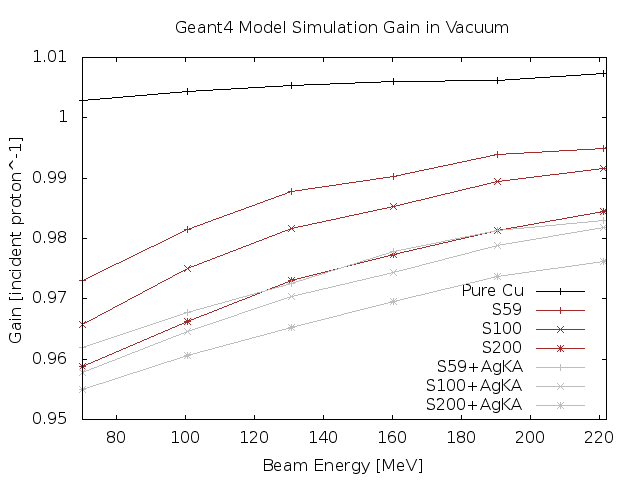
\includegraphics[width=0.77\linewidth]{figures/G4_gain.png}
\captionof{figure}{G4 gain output.  Kapton thickness proportionately negatively contributes; Ag ground layer suppresses Kapton behavior}
\end{center}

\begin{center}
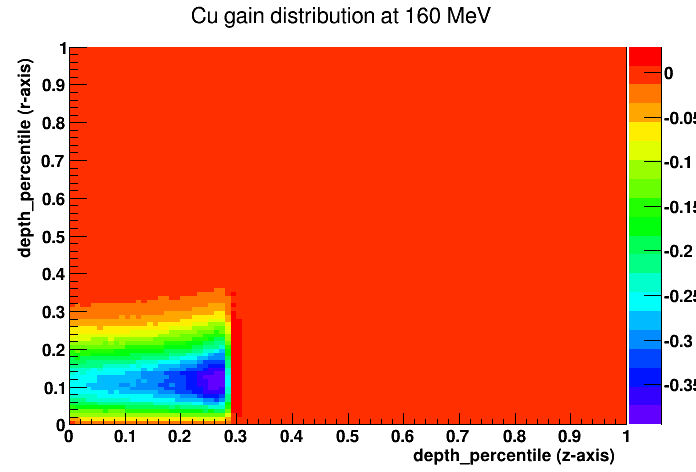
\includegraphics[width=0.77\linewidth]{figures/G4_gainCu_160MeV.png}
\captionof{figure}{G4 gain distribution map.  Electrons / ions straggle behind beam; inteface condition dependent upon energy (not shown).}
\end{center}

\begin{center}
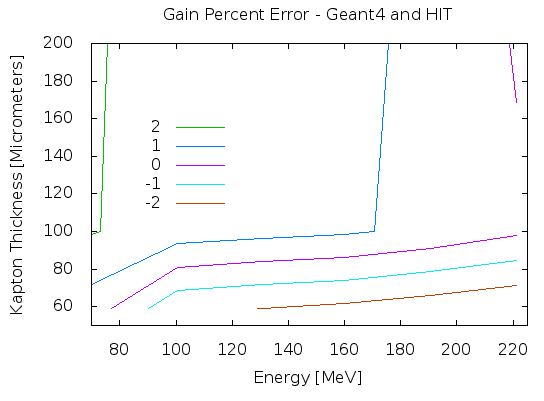
\includegraphics[width=0.77\linewidth]{figures/G4_HIT_error.png}
\captionof{figure}{Percent error contours between simulation and experiment gain measurement}
\end{center}
}

%----------------------------------------------------------------------------------------
%	Conclusions
%----------------------------------------------------------------------------------------

\headerbox{Discussion}{name=conclusions,column=3,row=0,aligned=introduction}{

\begin{itemize}[leftmargin=*]
\item {\fontsize{15}{18}\selectfont Optimal cup height, radius determined by coarse-grain MCNP6 model}
\item {\fontsize{15}{18}\selectfont Deposition close to Cu\\interface (low E) results in greater backscatter}
\item {\fontsize{15}{18}\selectfont -Ag/KA models acquire $\sim$0\% charge defect at\\finite Kapton thickness for various energies}
\item {\fontsize{15}{18}\selectfont \lq\lq Tertiary" electrons from (p,NpMn) reactions contribute non-linearly}
\end{itemize}
}

%----------------------------------------------------------------------------------------
%	CONTACT INFORMATION
%----------------------------------------------------------------------------------------

\headerbox{$^\dag$Contact Information}{name=contact,column=3,above=bottom}{

\begin{description}\compresslist
\item[Web] www.wpi.edu/$\sim$shaun
\item[Email] shaun@wpi.edu
\item[Phone] 
\end{description}
}

%----------------------------------------------------------------------------------------
%	REFERENCES
%----------------------------------------------------------------------------------------

\headerbox{References}{name=references,column=3,above=contact,below=conclusions}{

\renewcommand{\section}[2]{\vskip 0.05em} % Get rid of the default "References" section title
\nocite{*} % Insert publications even if they are not cited in the poster
\small{ % Reduce the font size in this block
\bibliographystyle{unsrt}
\bibliography{refs} % Use refs.bib as the bibliography file
}}

\end{poster}

\end{document}

%%%%%%%%%%%%%%%%%%%%%%%%%%%%%%%%%%%%%%%%%%%%%%%%%%%%%%%%%%%%%%%%%%%%%
% baposter Class Created by:
% Brian Amberg (baposter@brian-amberg.de)
%
% License:
% CC BY-NC-SA 3.0 (http://creativecommons.org/licenses/by-nc-sa/3.0/)
%%%%%%%%%%%%%%%%%%%%%%%%%%%%%%%%%%%%%%%%%%%%%%%%%%%%%%%%%%%%%%%%%%%%%
